\section{Background\textsuperscript{2}}
\bgroup
\def\arraystretch{2}% 
\begin{table*}[t]
\caption{Comparison of distributed ledger technologies (July 2018), extended from \cite{pustivsek2018approaches}}
\begin{tabu} to \textwidth {lXXXX}
   \toprule
 & Bitcoin & Ethereum & Hyperledger Fabric & IOTA \\ \midrule
 Native cryptocurrency & Yes & Yes & No & Yes \\
 Decentralized applications & No & Yes & Yes & No \\
 Transaction fee & Yes & Yes & No & No\\
Transaction fee/speed & \$0.15 / 10 min.\cite{bitcoinfees:online} & \$0.28 / 2 min.\cite{ethgasstation:online} & Instant & 5 min\cite{tanglemonitor:online}\\ 
 Transactions per sec. & 3-7 & 7-15 & 3500 \cite{androulaki2018hyperledger} & 10 \\ 
 Network type & Public & Public / Private  & Private & Public \\ 
 Network access & Permissionless & Permissionless & Permissioned & Both \\ 
 Anonymous accounts & Yes & Yes & No & Both \\ 
 State channels & Lightning & \mu Raiden, Raiden & Not required & Flash channels \\ 
 Suitable for IoT & No & With constraints  & Yes & Yes\\ 
 Suitable for DApps & No & Yes & Yes & No \\ \bottomrule
\end{tabu}
\raggedright {}
\label{table:dl_comparison}
\end{table*}
\egroup
Blockchain platforms in general provide a distributed data structure, the blockchain and a consensus mechanism, which allows to find a mutual agreement about the state of the blockchain. The blockchain data structure consists of blocks, were all transactions are stored in, and additionally contain a hash of the previous block. (Fig. \ref{fig:blockchain})
The basis of these system is, that every participant involved, stores the entire blockchain history, a manipulation of the state would require to alter data on the majority of system peers.
\begin{figure}[h]
    \centering
    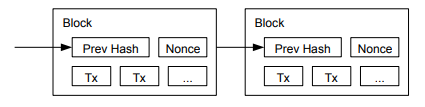
\includegraphics[width=0.5\textwidth]{assets/blockchain.png}
    \caption{Blockchain structure}
    \label{fig:blockchain}
\end{figure}
Blockchain is only one type of Distributed Ledger Technology (DLT), in a later section we will describe IOTA as another approach, which does not rely on the linear blockchain data structure.
The blockchain-based cryptocurrencies Bitcoin, Ethereum and Co. allow the settlement of financial transactions via a distributed, trusted ledger stored within the blockchain. 
But one of the most obstructive properties of these \\ blockchain-based systems, for Internet-of-Things (IoT) and micro-payment systems in general, is the occurrence of transaction fees and the required storage capacity to persist the distributed ledger.
IoT devices equipped with temperature and humidity sensors for example, continuously transmit a stream of small data packages. Thus, the usage of popular public block-chain systems e.g. Bitcoin or Ethereum, which incorporate transaction fees as a means for preventing transaction spam, is not economically viable. For use cases that are not built around a high distrust of every participant involved, permissioned blockchain solutions seem to be a promising approach, because consensus of transaction history is reached by a limited amount of peers. The blockchain data structure is the most popular Distributed Ledgers Technology (DLT). Recently an entire different architecture in form of the cryptocurrency IOTA emerged, which has been developed for IoT device use cases. It does not incorporate transaction fees and does not suffer from typical blockchain scalability problems. In Table \ref{table:dl_comparison} we compare the properties of different distributed ledger technologies side-by-side, additionally we provide a deeper explanation of these technologies in the following sections. 

\subsection{Bitcoin}
Bitcoin, proposed 2007 by the pseudonym Satoshi Nakamoto, was the first cryptocurrency, which solved the double spending problem by a distributed network consensus mechanism. In its initial design, Bitcoin has a very limited smart contract capability. Smart contract code needs to be executed by every node for verification, which entails the risk that a given code might be too computational expensive and slow down or even halt the network. While Ethereum, as described in the following section, counters this problem with defined costs for every computational operation performed, Bitcoin was not designed with these capabilities at its inception.
\\ \\
As other blockchain platforms, Bitcoin also suffers from a transaction bottleneck, mainly caused by a system design that enforces the generation of a new block roughly every 10 minutes and the fixed maximum block size of 1 Megabyte, which limits the number of transactions a block can hold. This bottleneck, resulted in peaks with high numbers of unprocessed transactions and fees of over 50 Dollar in December 2017 \cite{bitcoin-txfee:online} for a single transaction.
To circumvent these limitations, numerous blockchain forks emerged, which either increase the block size limit, reduce the block time, or both.\\ \\
While numerous proposals exist to extend Bitcoins capabilities regarding transaction throughput or scalability in general, these proposals are still not in widespread use or not yet completed.\cite{poon2016bitcoin}

\subsection{Ethereum}
Ethereum was developed upon the core principles of the Bitcoin protocol, while extending it in various ways that were not foreseeable at the introduction of Bitcoin and optimizing it for mass adoption. One of the shortcomings of Bitcoin, was the lack of a Turing-complete programming language to allow smart contracts. Smart Contracts
enable a the transparent implementation of business logic on a blockchain for all participants who want to interact with it.
Ethereum implemented the Ethereum Virtual Machine (EVM) which handles internal state, computation and allows smart contracts to be deployed to the blockchain. Transactions can not only be send to other users but also to smart contracts, where they invoke contract functions, which in turn could invoke other smart contracts themself.
\\
The extensive smart contract capabilities resulted in the tokenization of various assets and the ability to trade them on the Ethereum network. \\ \\
With the ERC-20 token standard, which provides common rules for token transfers, interaction and made it easy to implement and issue tokens, a multitude of token smart contracts emerged. Today, about 99,000 known ERC token contracts exist on the Ethereum blockchain \cite{Etherscan1:online}, many of them providing services based on these tokens. The widespread adoption of ERC tokens and related services has led to the largest community and development ecosystem for smart contracts to date.
\\
To solve different scalability problems, numerous side projects are under development to provide off-chain solutions \cite{eberhardt2017or} or extend Ethereums capabilities, similar to Bitcoin.

\subsection{IOTA}
IOTA is a cryptocurrency introduced in 2016 \cite{popovtangle:online}, which does not use a typical blockchain data structure. It uses a data structure, called \textit{Tangle}.
\begin{figure}[ht]
\centering
  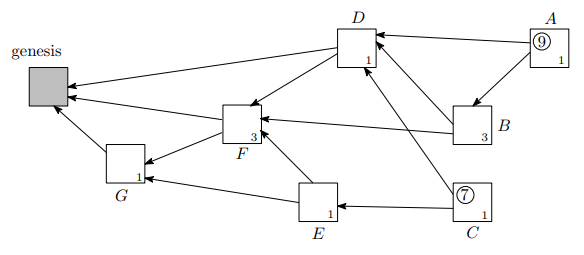
\includegraphics[width=0.5\textwidth]{assets/tangle.png}
\caption{Tangle data structure}
\label{fig:tangle}
\end{figure}
As depicted in Figure \ref{fig:tangle}, every transaction validates two former transactions. In this system, more activity in the IOTA network leads to faster validation and confirmation of transactions and theoretically unlimited scalability.
\\
While the  blockchain architecture of Bitcoin and Ethereum with their finite block size and enforced block time, limits the number of transaction in a certain time frame, IOTA does not have these constraints. But the advantages of IOTAs architecture only become apparent when a certain size of the network is reached. It is designed as a protocol for the rapidly rising number of IoT devices, for a machine-to-machine (M2M) economy, where devices interact with each other autonomously. In this regard, IOTA would be an enabler for the processing of a tremendous amount of transactions. Currently, the IOTA network handles about 10 transactions per second while after a stress test at the end of the year 2017 the IOTA team reported 100 transactions per second. As mentioned earlier, theoretically IOTA is able to outperform blockchain based technologies, if the network size i.e. the transaction throughput, reaches a certain threshold. \\

The IOTA Foundation itself describes various future use cases for IOTA: Over-the-air updates for IoT devices, data marketplaces, supply-chain management and more.
IOTA is an interesting approach, with its clear focus on IoT devices and enabling a machine-to-machine economy, in this early stage of the IOTA network, however, it is not an ideal solution for instant payments.\\

\subsection{Hyperledger Fabric}
Hyperledger Fabric is a permissioned blockchain framework initially developed by IBM and now part of the Linux Foundation. As a framework, it is not a single blockchain, but a basis to develop blockchain solutions for enterprise ecosystems \cite{androulaki2018hyperledger}. Contrary, to the other proposed solutions, it does not include a native cryptocurrency. Its Byzantine-fault tolerant (BFT) consensus mechanism \cite{castro1999practical} is designed for an environment where all participants are explicitly identified and have a common goal in general, which does not imply that all parties trust each other fully. Besides, the default consensus mechanism is replaceable, to allow different approaches depending on use case. For smart contracts, Fabric allows the usage of standardized programming languages (Go, NodeJS, Java) and does not integrate its own language, hence the project describes itself as "the first distributed operating system for permissioned blockchains" \cite{androulaki2018hyperledger}.
\\
Fabrics \textit{membership service provider} (MSP) is responsible for authentication of all network participants, it issues cryptographic certificates for interaction with the network and checks their validity. The network can be governed by multiple MSPs, in many Fabric implementations this is a committee representing all stakeholders.
\\ \\
On the Fabric platform, every smart contract (in Fabric terms: chaincode) runs in its own docker container, separated from other chaincodes or the host system. Additionally, by design, the host system is agnostic of the chaincodes underlying programming language.
\\ \\
Fabric also integrates the concept of (transaction) channels, which allows fine-grained control about which transaction information is visible to participants. With this, confidential transactions can take place on the Fabric blockchain, while complying with f.g. legal restrictions.
By design, the chaincode is not inevitably executed by every peer of the system, this is a matter of individual configuration (endorsement policy), which can significantly increase the overall transaction throughput of the system, compared to Bitcoin or Ethereum, where execution is required by every peer.